\documentclass[12pt,letterpaper]{article}
\usepackage{graphicx}
\usepackage[letterpaper,margin=0.75in]{geometry}

\usepackage{xcolor} % Required for specifying custom colours
\definecolor{grey}{rgb}{0.9,0.9,0.9} % Colour of the box surrounding the title

\usepackage[utf8]{inputenc} % Required for inputting international characters
\usepackage[T1]{fontenc} % Output font encoding for international characters
\usepackage[sfdefault]{ClearSans} % Use the Clear Sans font (sans serif)

\usepackage{calc}

\usepackage{tikz}
\usepackage{xstring}
\usepackage{siunitx}
\usepackage{appendix}
\usepackage{multirow}
\usepackage{longtable}

\overfullrule=5pt

\begin{document}
\newcommand{\getx}[1] {\StrBetween{#1}{(}{,}}
\newcommand{\gety}[1] {\StrBetween{#1}{,}{)}}
%\newcommand{\unpair}[2] {\expandafter\def#2{\getx {#1}}}
\def\mydef#1#2{\def#1{#2}}
\def\uncoord#1#2#3{\def#2{\getx{#1}}\def#3{\gety{#1}}}

\newcommand{\busline}[2] {\draw[thick] #1--#2;}

%----------------------------------------------------------------------------------------
%	TITLE PAGE
%----------------------------------------------------------------------------------------

\begin{titlepage} % Suppresses displaying the page number on the title page and the subsequent page counts as page 1
	
	%------------------------------------------------
	%	Grey title box
	%------------------------------------------------
	
	\colorbox{grey}{
		\parbox[t]{0.93\textwidth}{ % Outer full width box
			\parbox[t]{0.91\textwidth}{ % Inner box for inner right text margin
				\raggedleft % Right align the text
				\fontsize{50pt}{50pt}\selectfont % Title font size, the first argument is the font size and the second is the line spacing, adjust depending on title length
				\vspace{0.6cm} % Space between the start of the title and the top of the grey box
				
				Power Seat \\ 
				Wiring Harness\\
				\vspace{0.6cm} % Space between the end of the title and the bottom of the grey box
			}
		}
	}

	\parbox[t]{0.93\textwidth}{
		\raggedleft
	    \vspace{0.7cm}
		\textit{Project goals, dimensions, parts list, cost breakdown, and wiring diagram.}
	}
	\center
    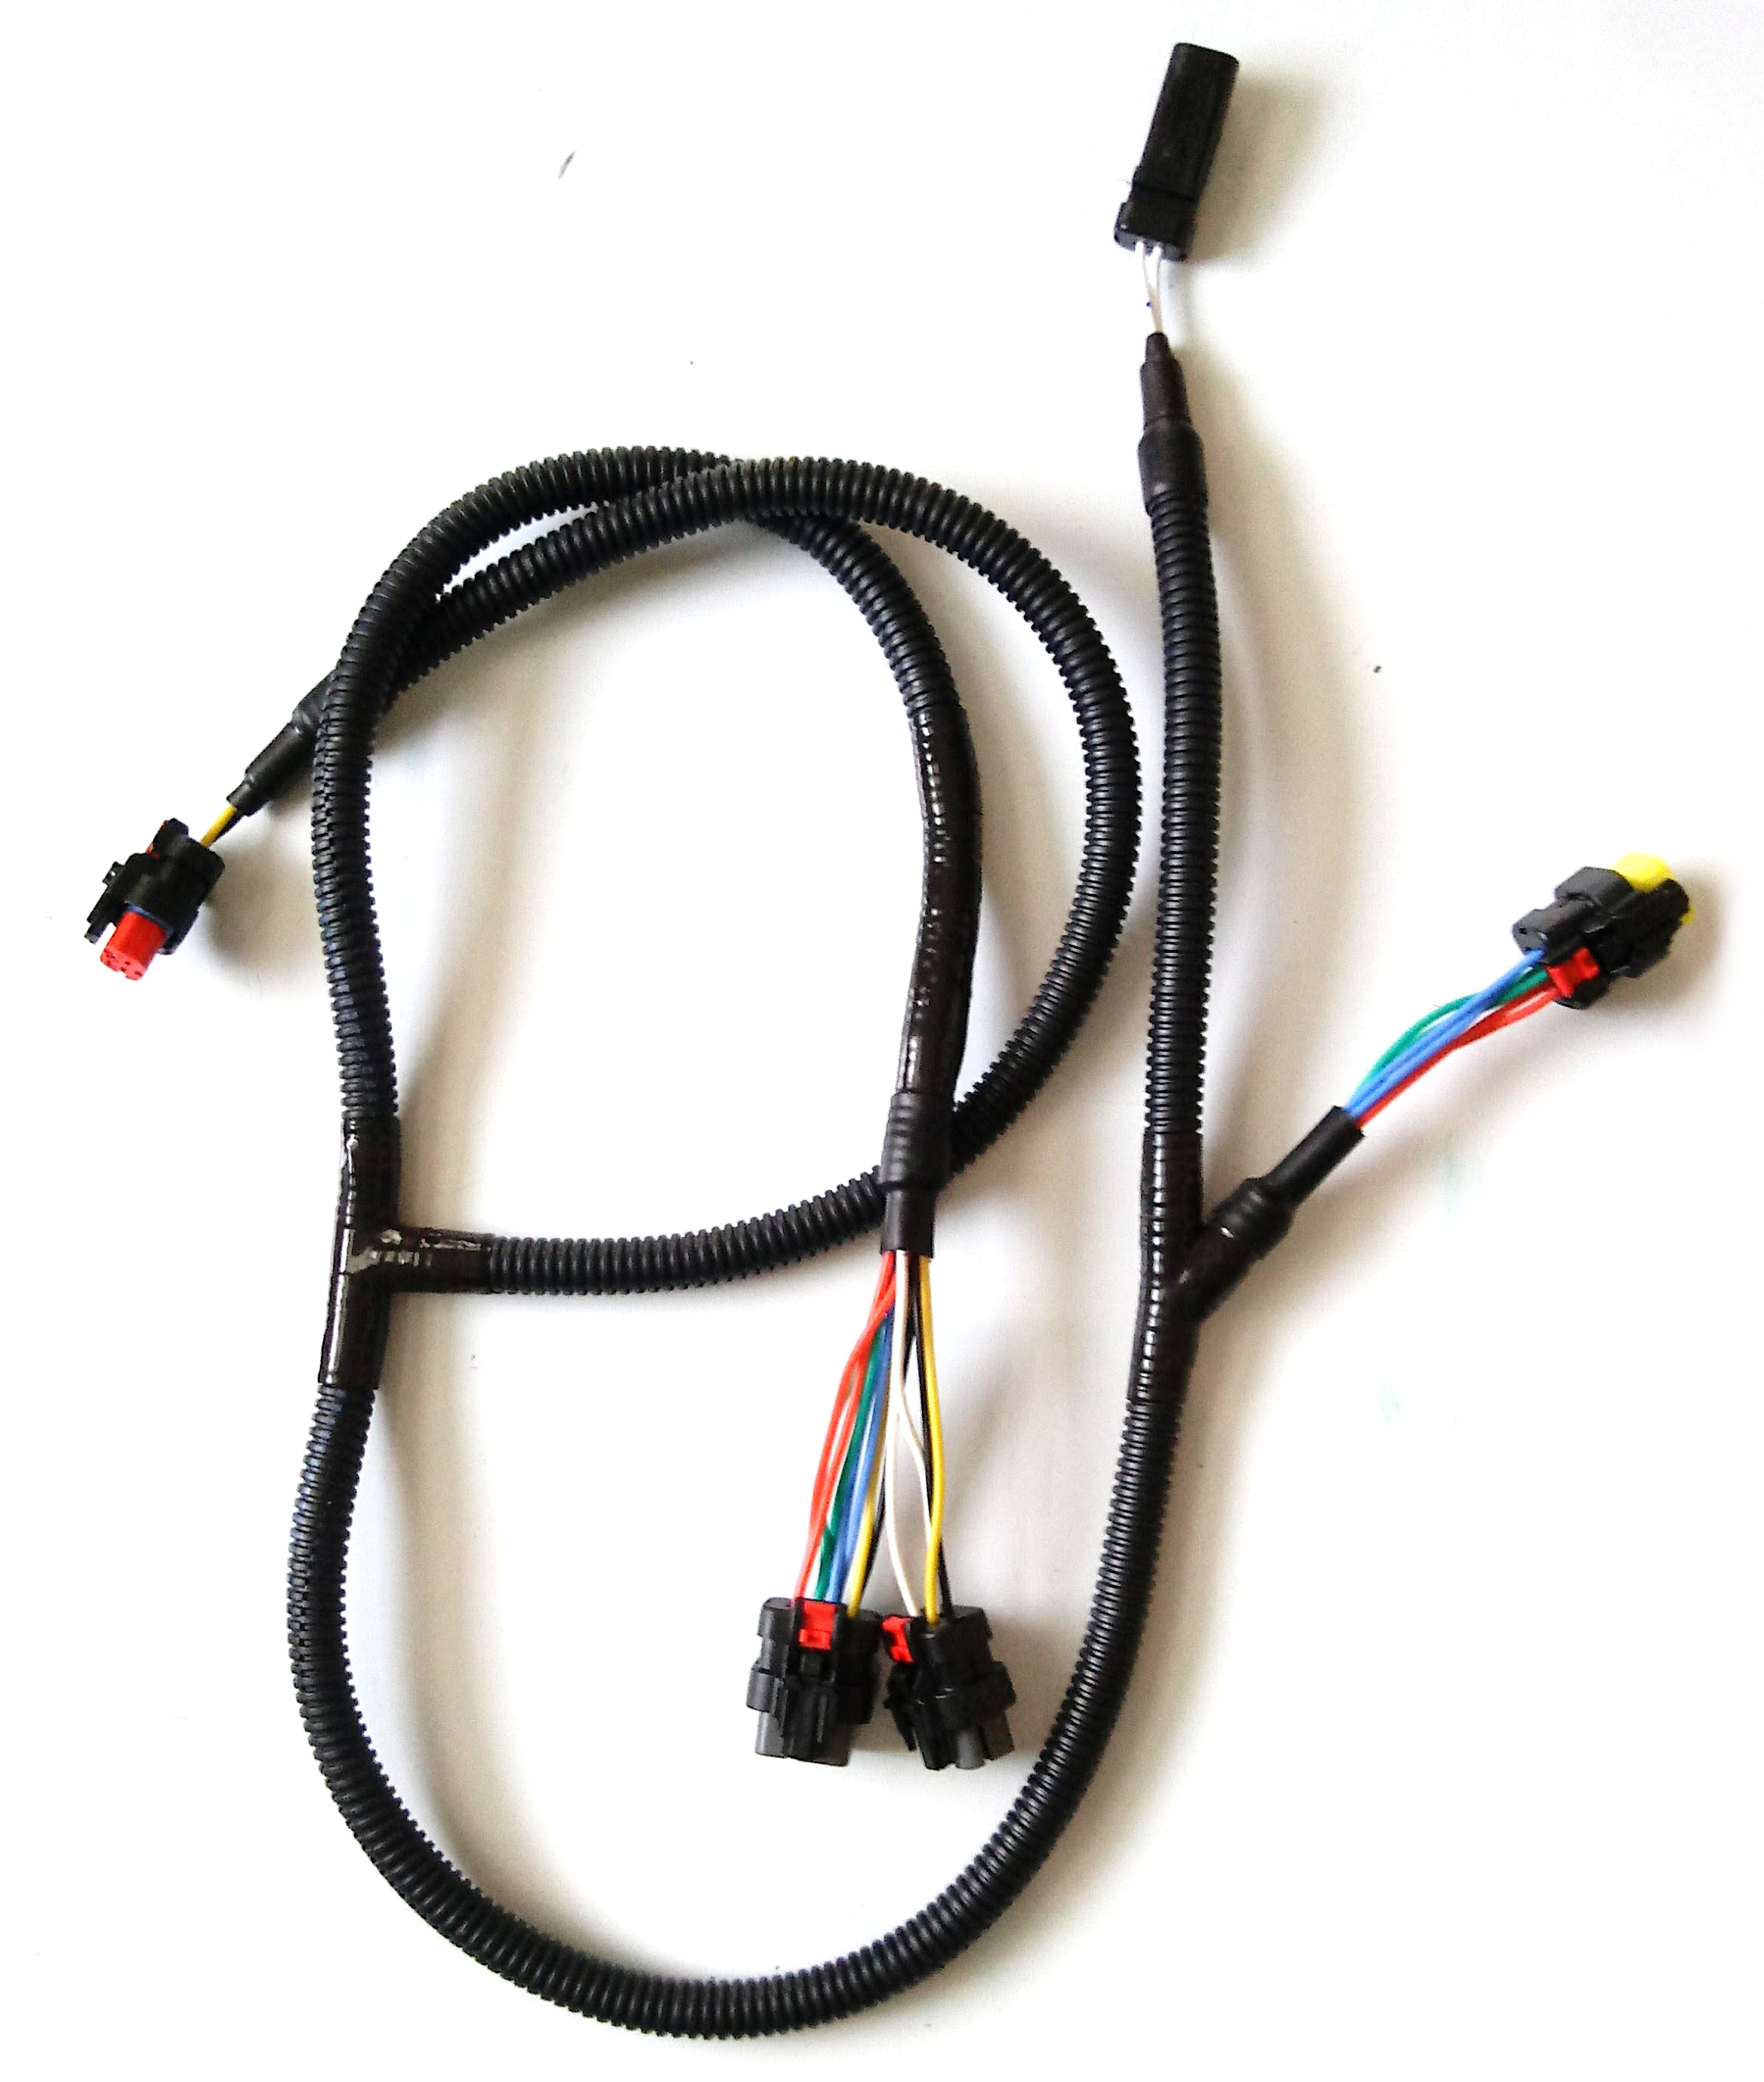
\includegraphics[width=0.80\linewidth]{1122171514.jpg}

	\vfill % Space between the title box and author information
	
	%------------------------------------------------
	%	Author name and information
	%------------------------------------------------
	
	\parbox[t]{0.93\textwidth}{ % Box to inset this section slightly
		\raggedleft % Right align the text
		%\hfill\rule{0.247\linewidth}{1pt}\\% Horizontal line, first argument width, second thickness
		\textit{
		  Vlad Shcherbakov \\
		  November 2017
		}
		
		%\hfill\rule{0.247\linewidth}{1pt}% Horizontal line, first argument width, second thickness
	}

	
\end{titlepage}
\newgeometry{left=0.75in,right=0.75in,top=1in,bottom=0.75in}
\section{Overview}
The goal of this project is to design a power seat harness for a hypothetical 8-way automotive power seat. It will not fit any particular car, and is constructed purely as a prototype. However it should highlight the issues that arise in the design of any wiring harness.

Power seats use electrical motors to control seat’s relative positioning within the car, as well as its overall shape. Power controls are often combined with additional manual adjustment mechanisms. The type of a power seat is usually specified by quantifying the number of ways it can be adjusted using power controls. This number does not include the number of ways a seat can be adjusted using manual controls and does not alone specify which controls are manual and which are powered. Thus not all 8-way power seats are alike.

Our hypothetical power seat, will have power adjustable \textit{bottom height}, \textit{bottom angle}, \textit{seat distance} from the steering wheel and \textit{lumbar support}. That’s total of 4 adjustable parameters. Since each one of the 4 parameters can be adjusted in 2 ways(increased or decreased) there are total of 8 ways in which seat can be adjusted. In addition to 4 power adjustments, there’s going to be one more manual adjustment: \textit{seatback recline}.
% \begin{figure}[b!]
%   \centering
%   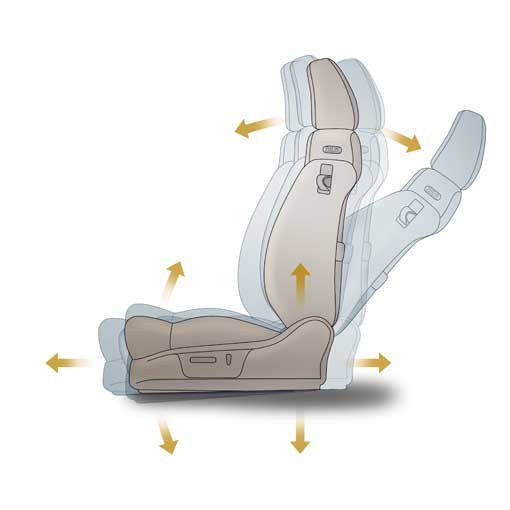
\includegraphics[width=0.70\linewidth]{8-way-seat.jpg}
%   \caption{8-way power seat with manual backseat recline adjustment.}
%   \label{fig:wireharness1}
% \end{figure}

\section{Requirements}
The role of the power seat wiring harness is to conduct electrical current between \textit{power source}, mechanical \textit{switch assemblies} and electrical \textit{motors}. Our power seat uses \textit{4 electrical motors} and \textit{2 switch assemblies}. The switch assemblies control which electrical motors receive electrical current as well as in which direction it is flowing for each motor.

The first switch assembly is used just for \textit{lumbar support} and controls only one motor, while the second switch assembly controls the other 3 motors, for \textit{height}, \textit{angle} and \textit{distance} adjustments.

The motors used are all \textit{Direct Current(DC)} and each is a two-terminal device. Each motor is usually dedicated to adjusting a single parameter, with the exception of \textit{angle} and \textit{height}. Neither of those two parameters are controlled by any single motor, but by two motors working in tandem: one raises(or lowers) the front and the other raises(or lowers) the back of the seat.

The power is supplied from without by a lead-acid battery over two terminals, usually with 12\si{\volt} potential between them and hopefully with a fuse somewhere in series as the only current limiting device. 

In order for motors to be able to turn in either direction they must be connected in such a way that the polarities of the potentials applied to their two terminals could be inversed. This could not be true, for example, if one of the terminals was always connected to ground! That means there will be two wires leading from each motor to the respective switch assembly.

Likewise, to be able to control direction of rotation of the motors, each switch assembly requires two power inputs, for both ground and positive potential, meaning a total of 4 power lines is needed. This is a problem, because the power terminal of the car supplies only 2. Additional 2 power lines will have to be spliced from the 2 existing ones in order to supply power for the second switch assembly.

\newpage
\newgeometry{margin=0.75in}
\section{Equivalent Circuit}

In order to better understand operation of the mechanical switch assemblies it is helpful to consider an equivalent circuit using a commonplace Double-Pole, Double-Throw or DPDT On-Off switch as shown in Figure 1. The motor will change direction when the switch is flipped.
%\vfill
\begin{figure}[h]\label{fig:motorcontrol}
\centering
%\def\svgwidth{0.62\columnwidth}
\def\svgscale{0.4}
\input{motorcontrol.pdf_tex}
\caption{Equivalent circuit for a switch assembly using DPDT On-Off switch}
\end{figure}

\section{Layout}
Figure 2 on the next page outlines the general layout of the wiring harness as well as exact dimensions of different sections. Black lines indicate sections of wires protected by plastic loom, gray lines are unprotected wire sections.

% \begin{figure}[h]\label{fig:motorcontrol}
% \centering
% %\def\svgwidth{0.62\columnwidth}
% \def\svgwidth{0.61\linewidth}
% \input{layout.pdf_tex}
% \caption{Equivalent circuit for a switch assembly using DPDT On-Off switch}
% \end{figure}

\begin{figure}[h!]
  \centering
  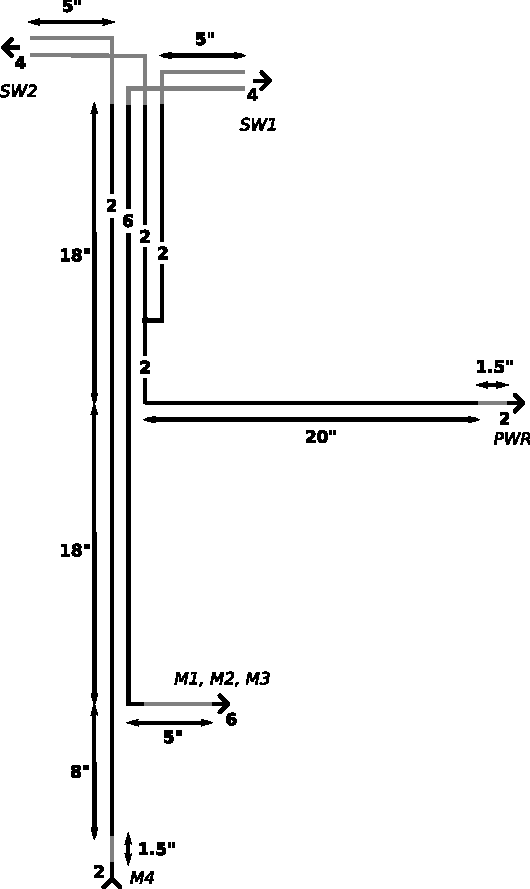
\includegraphics[width=0.75\linewidth]{layout.pdf}
  \caption{Layout of the wiring harness}
  \label{fig:layout}
\end{figure}

% \begin{figure}[h!]
%   \centering
%   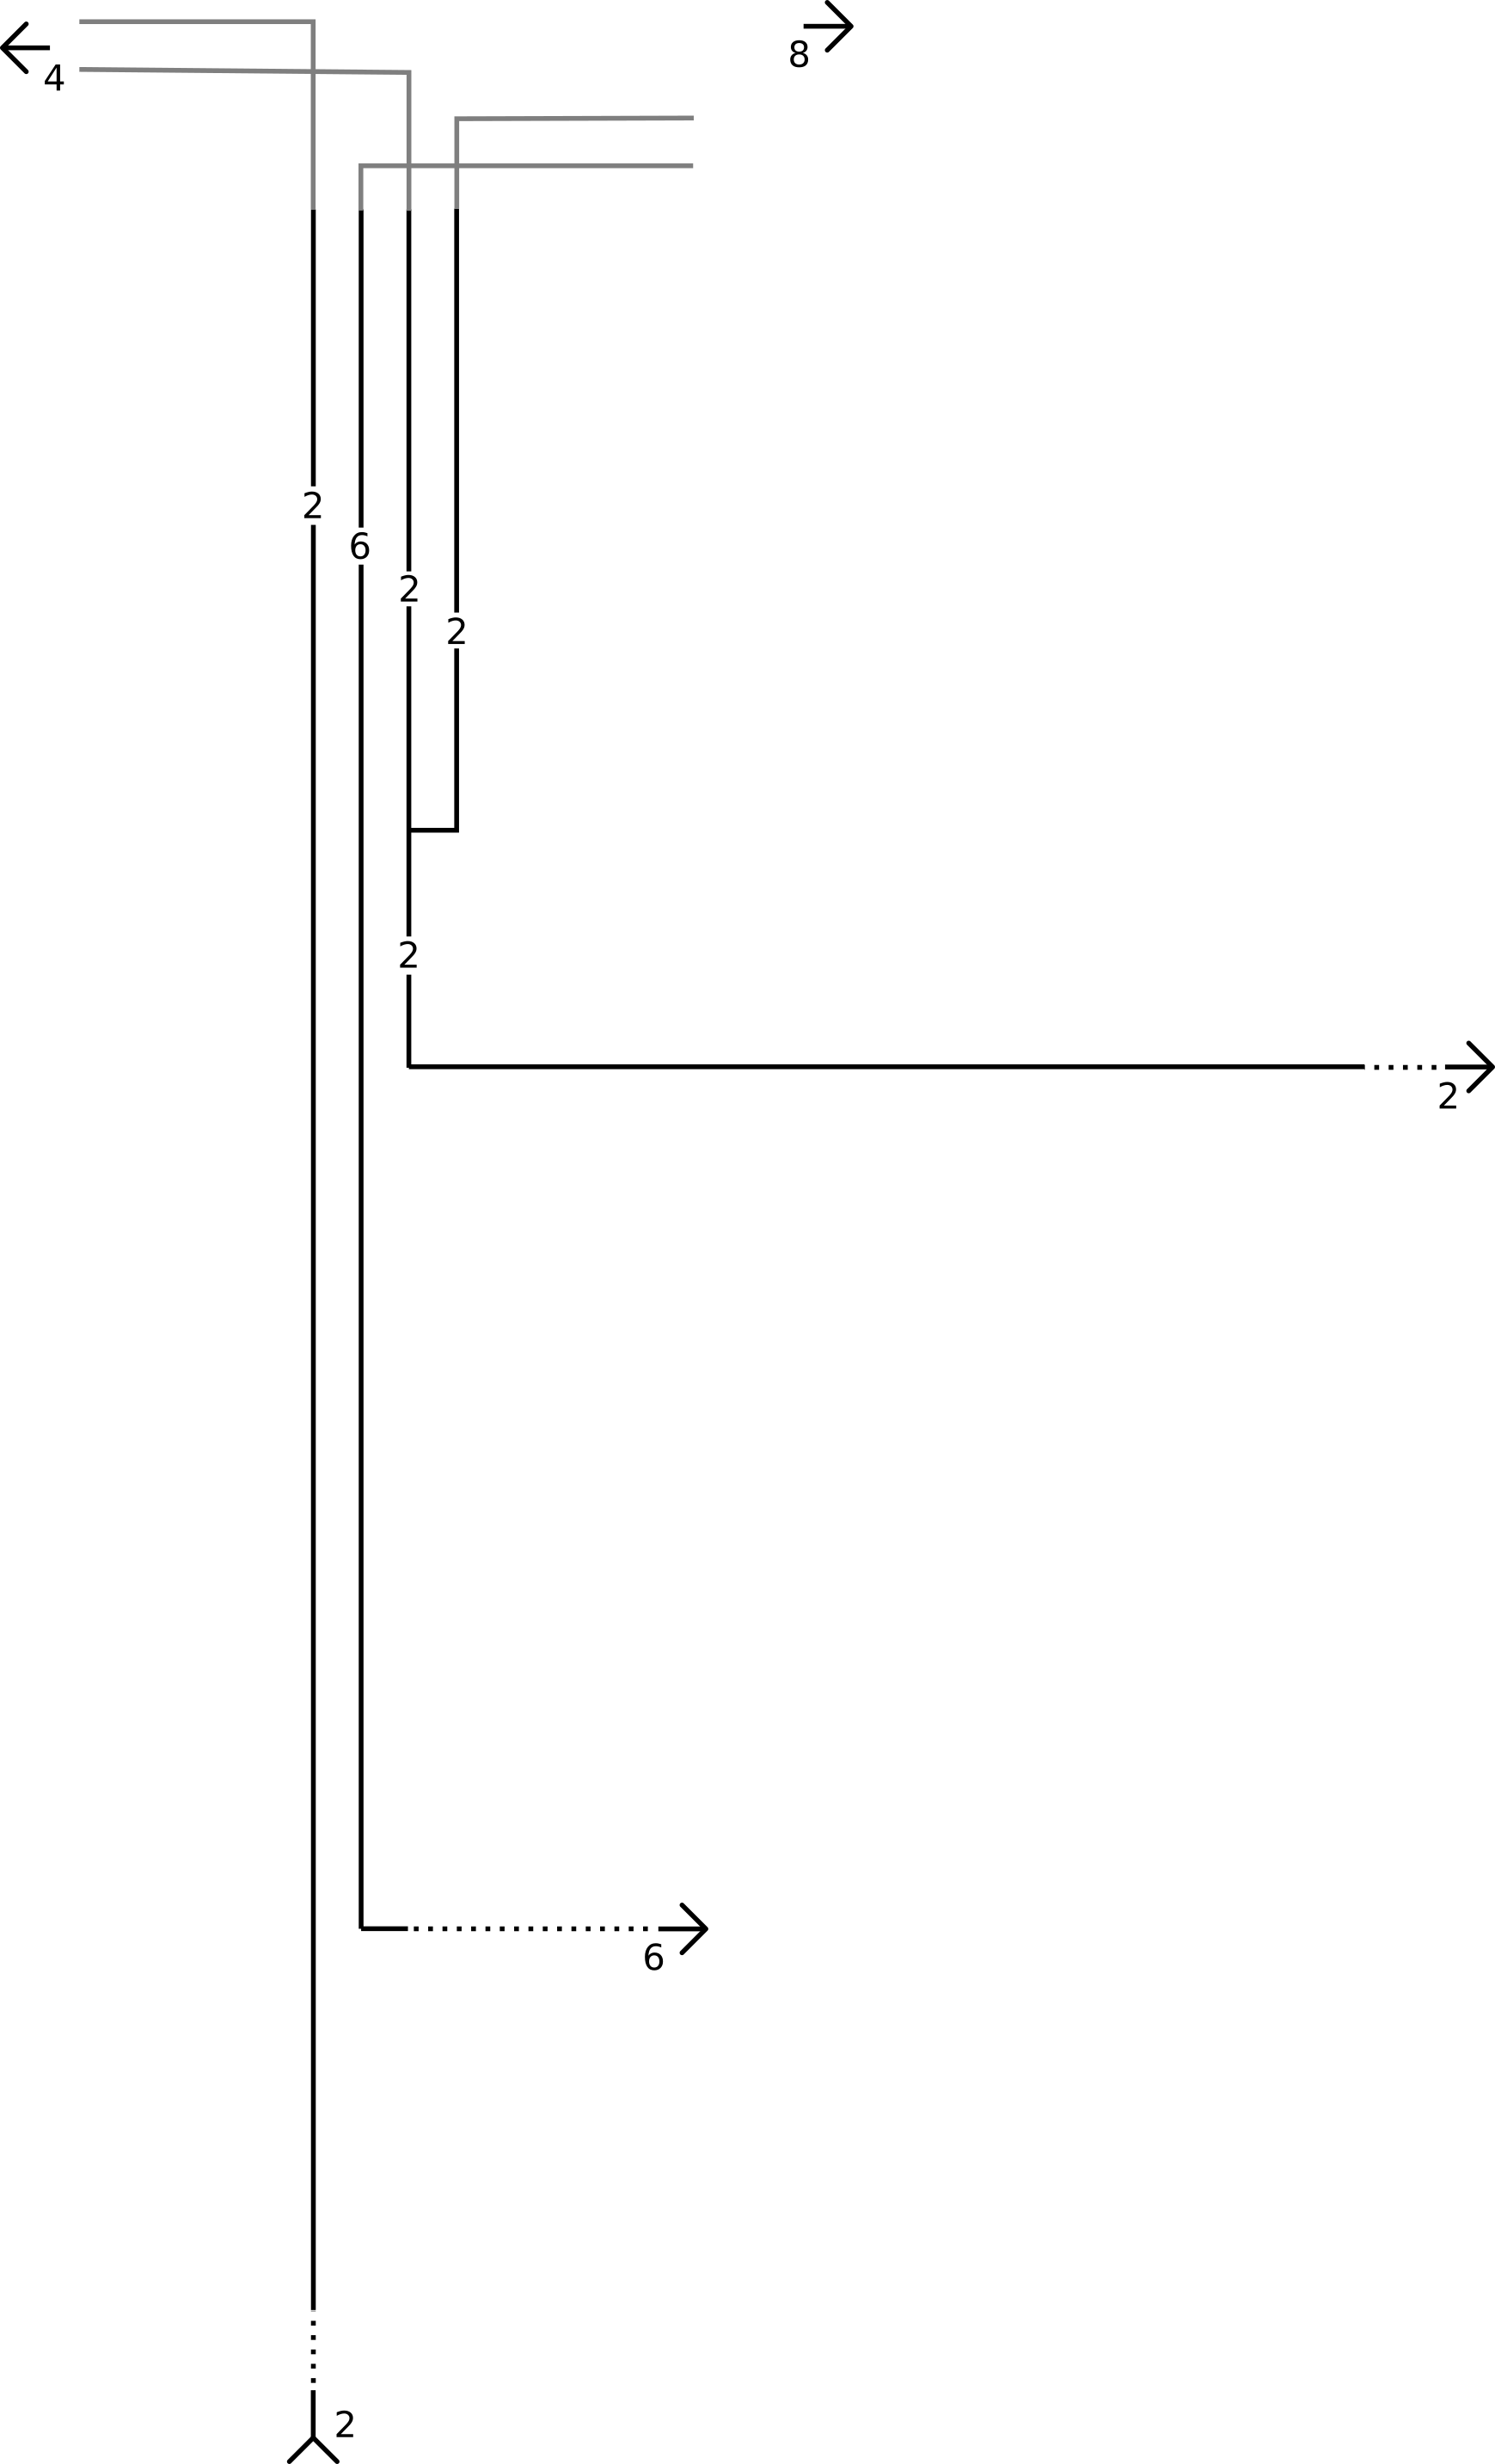
\includegraphics[width=0.73\linewidth]{layout.png}
%   \caption{Layout of the wiring harness}
%   \label{fig:wireharness1}
% \end{figure}

\newpage
\section{Materials}
This section lists all the parts required to assemble the harness. Where materials need to be cut to specific lengths(such as wires and plastic tubes), all cut lengths are specified.

% The connector housing used for this harness are all from AMPSEAL 16 series made by TE Connectivity. They were chosen for their rugged construction, environmental sealing and locking features. 

% To protect the wires, 3/8" flame-retardant convoluted split plastic tubing was used. The single diameter was big enough to hold up to 12 of 18 AWG wires in the thickest parts, like near the switch assembles, and thin enough to hold down to 2 wires snugly in power source and lumbar motor sections.

% Heat shrunk rubber tubing was used to terminate the ends of the plastic loom tubing. Where a single heat shrink tube wouldn't have enough shrink ratio to hold down a bundle of wires reliably, a two stage approach was utilized made up of a piece of 3/4" and of 3/8" shrink tube sections. 

% Use of tape was minimized on purpose, as it is usually the first component to fail and wear out under stress. The only two important places where tape was used are the T-section and a Y-branch. There a special non-adhesive silicone tape was used: it's a kind of tape that only sticks to itself. It is difficult to work with, but it's main advantage is it's clay-like ability to conform to any shape and it's python-strong grip with itself once it fuses.

% The wire used for this harness is a cheap hook up wire, because it was cheaper to buy it as a set of different colors. A more reliable primary wire should be used for a real wire harness.

\begin{longtable}{c l}

\parbox[c]{4cm}{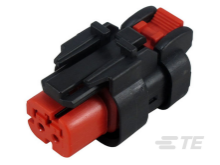
\includegraphics[width=4cm]{776427-1.png} }
& \begin{tabular}{l l}
\textbf{Part Number:} 776427-1 & \textbf{Connector Style:} Male \\
\textbf{Manufacturer:} TE Connectivity & \textbf{Unit Price:} \$0.85 \\
\textbf{Number of Positions:} 2 & \textbf{Quantity:} 1 \\
\textbf{Product Series:} AMPSEAL 16 & \textbf{Color:} Red \\
\multicolumn{2}{p{8cm}}{\textbf{Description:} Connector Housing } \\
\end{tabular} \\

\parbox[c]{5cm}{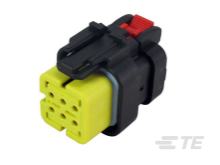
\includegraphics[width=5cm]{776531-3.png} }
& \begin{tabular}{l l}
\textbf{Part Number:} 776531-3 & \textbf{Connector Style:} Male \\
\textbf{Manufacturer:} TE Connectivity & \textbf{Unit Price:} \$1.46 \\
\textbf{Number of Positions:} 6 & \textbf{Quantity:} 1 \\
\textbf{Product Series:} AMPSEAL 16 & \textbf{Color:} Yellow \\
\multicolumn{2}{p{8cm}}{\textbf{Description:} Connector Housing } \\
\end{tabular} \\

\parbox[c]{5cm}{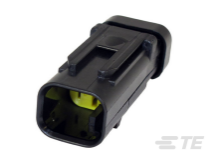
\includegraphics[width=5cm]{776534-3.png} }
& \begin{tabular}{l l}
\textbf{Part Number:} 776534-3 & \textbf{Connector Style:} Female \\
\textbf{Manufacturer:} TE Connectivity & \textbf{Unit Price:} \$1.06 \\
\textbf{Number of Positions:} 2 & \textbf{Quantity:} 1 \\
\textbf{Product Series:} AMPSEAL 16 & \textbf{Color:} Yellow \\
\multicolumn{2}{p{8cm}}{\textbf{Description:} Connector Housing } \\
\end{tabular} \\

\parbox[c]{5cm}{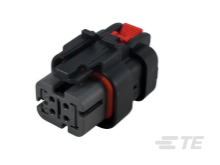
\includegraphics[width=5cm]{776524-2.png} }
& \begin{tabular}{l l}
\textbf{Part Number:} 776524-2 & \textbf{Connector Style:} Male \\
\textbf{Manufacturer:} TE Connectivity & \textbf{Unit Price:} \$1.50 \\
\textbf{Number of Positions:} 4 & \textbf{Quantity:} 1 \\
\textbf{Product Series:} AMPSEAL 16 & \textbf{Color:} Grey \\
\multicolumn{2}{p{8cm}}{\textbf{Description:} Connector Housing } \\
\end{tabular} \\

\parbox[c]{5cm}{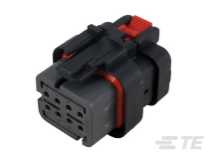
\includegraphics[width=5cm]{776532-2.png} }
& \begin{tabular}{l l}
\textbf{Part Number:} 776532-2 & \textbf{Connector Style:} Male \\
\textbf{Manufacturer:} TE Connectivity & \textbf{Unit Price:} \$2.06 \\
\textbf{Number of Positions:} 8 & \textbf{Quantity:} 1 \\
\textbf{Product Series:} AMPSEAL 16 & \textbf{Color:} Grey \\
\multicolumn{2}{p{8cm}}{\textbf{Description:} Connector Housing } \\
\end{tabular} \\

\parbox[c]{5cm}{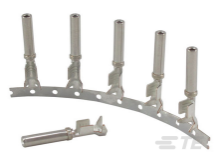
\includegraphics[width=5cm]{776492-1.png} }
& \begin{tabular}{l l}
\textbf{Part Number:} 776492-1 & \textbf{Wire Size (AWG):} 18-14 \\
\textbf{Manufacturer:} TE Connectivity & \textbf{Unit Price:} \$0.46 \\
\textbf{Terminal Style:} Socket & \textbf{Quantity:} 20 \\
\textbf{Product Series:} AMPSEAL 16 & \textbf{Current Rating (A):} 13 \\
\textbf{Description:} Socket Terminal  & \textbf{Pin Diameter:} 1.588\si{\milli\meter} \\
\end{tabular} \\

\parbox[c]{5cm}{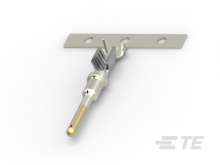
\includegraphics[width=5cm]{2098250-1.png} }
& \begin{tabular}{l l}
\textbf{Part Number:} 2098250-1 & \textbf{Wire Size (AWG):} 18-14 \\
\textbf{Manufacturer:} TE Connectivity & \textbf{Unit Price:} \$0.27 \\
\textbf{Terminal Style:} Pin & \textbf{Quantity:} 2 \\
\textbf{Product Series:} AMPSEAL 16 & \textbf{Current Rating (A):} 13 \\
\textbf{Description:} Pin Terminal  & \textbf{Pin Diameter:} 1.588\si{\milli\meter} \\
\end{tabular} \\

\parbox[c]{5cm}{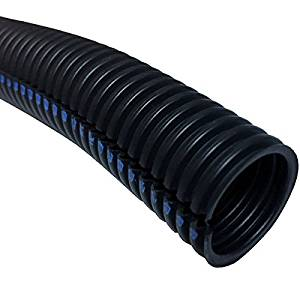
\includegraphics[width=5cm]{3by8loomtubing.jpeg} }
& \begin{tabular}{l l}
\textbf{Manufacturer:} Electriduct Inc & \textbf{Price per Inch:} \$0.12 \\
\textbf{Diameter:} 3/4" & \textbf{Cut Lengths:} 44", 20", 1" \\
\textbf{Description:} Split Wire Loom Tubing & \textbf{Total Lengths:} 65" \\
\end{tabular} \\

\parbox[c]{5cm}{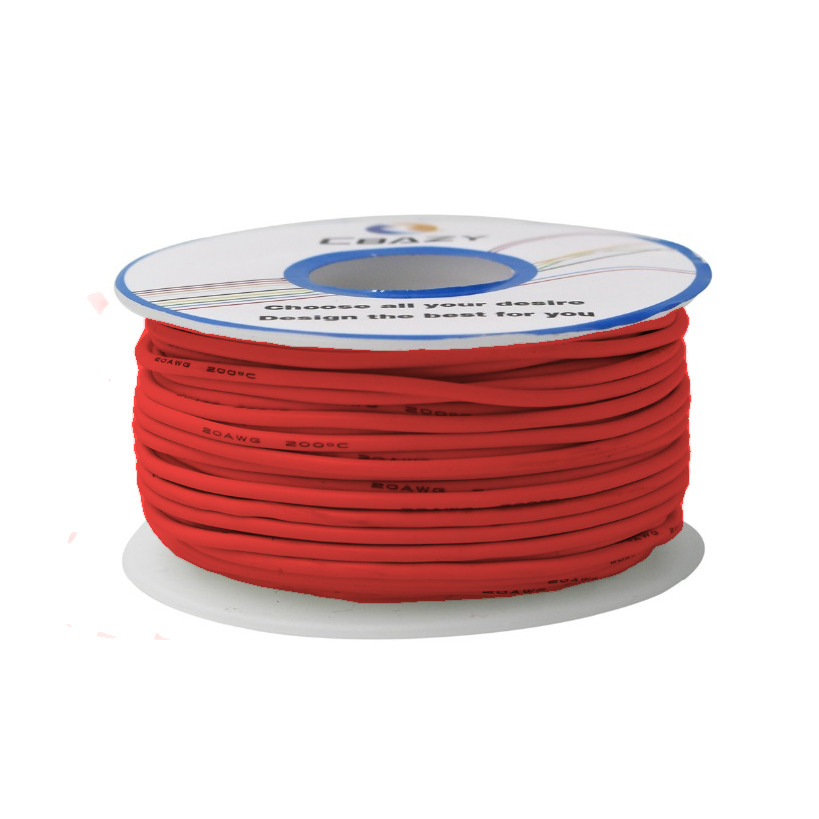
\includegraphics[width=5cm]{redwire.jpg} }
& \begin{tabular}{l l}
\textbf{Manufacturer:} CBAZY & \textbf{Price per Inch:} \$0.02 \\
\textbf{Size:} 18AWG & \textbf{Cut Lengths:} 46"x2 \\
\textbf{Color:} Red  & \textbf{Total Length:} 92" \\
\multicolumn{2}{p{8cm}}{\textbf{Description:} Stranded Hook-up Wire } \\
\end{tabular} \\

\parbox[c]{5cm}{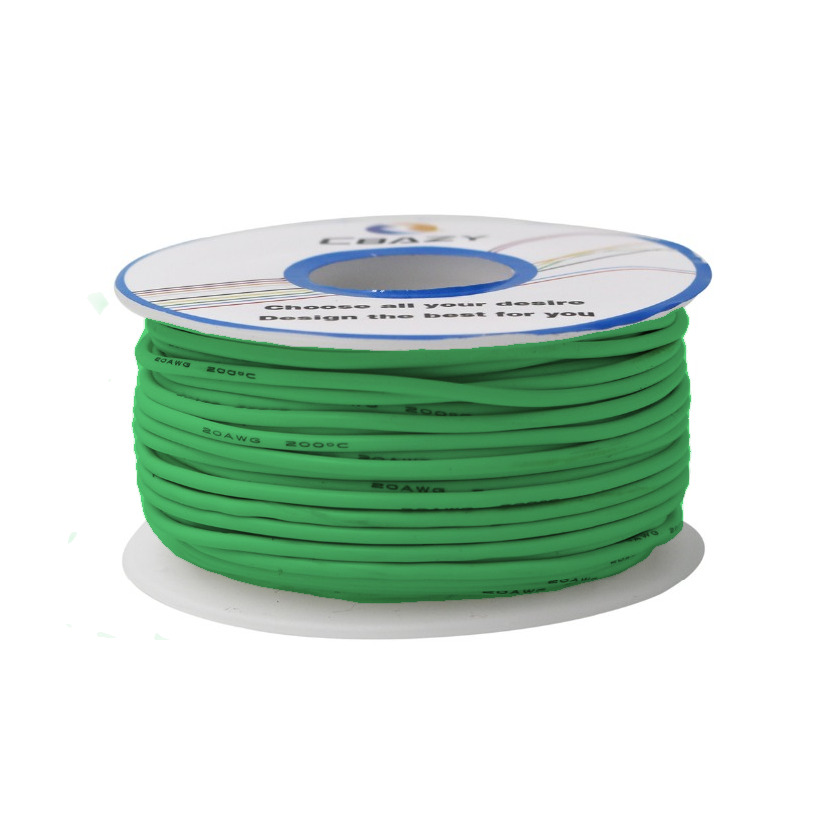
\includegraphics[width=5cm]{greenwire.jpg} }
& \begin{tabular}{l l}
\textbf{Manufacturer:} CBAZY & \textbf{Price per Inch:} \$0.02 \\
\textbf{Size:} 18AWG & \textbf{Cut Lengths:} 46"x2 \\
\textbf{Color:} Green  & \textbf{Total Length:} 92" \\
\multicolumn{2}{p{8cm}}{\textbf{Description:} Stranded Hook-up Wire } \\
\end{tabular} \\

\parbox[c]{5cm}{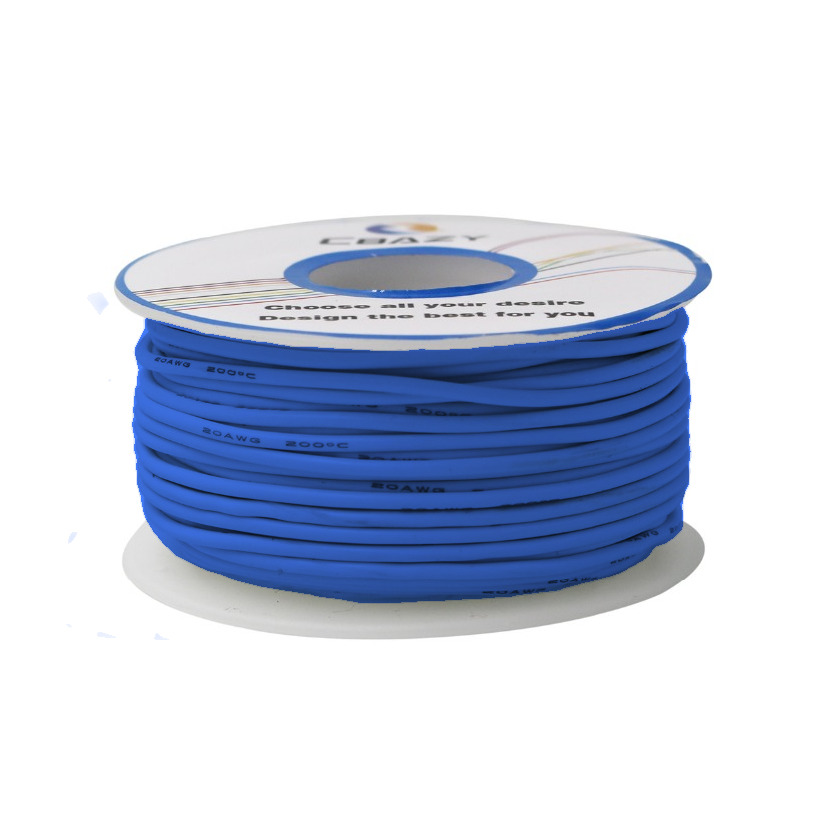
\includegraphics[width=5cm]{bluewire.jpg} }
& \begin{tabular}{l l}
\textbf{Manufacturer:} CBAZY & \textbf{Price per Inch:} \$0.02 \\
\textbf{Size:} 18AWG & \textbf{Cut Lengths:} 46"x2 \\
\textbf{Color:} Blue  & \textbf{Total Length:} 92" \\
\multicolumn{2}{p{8cm}}{\textbf{Description:} Stranded Hook-up Wire } \\
\end{tabular} \\

\parbox[c]{5cm}{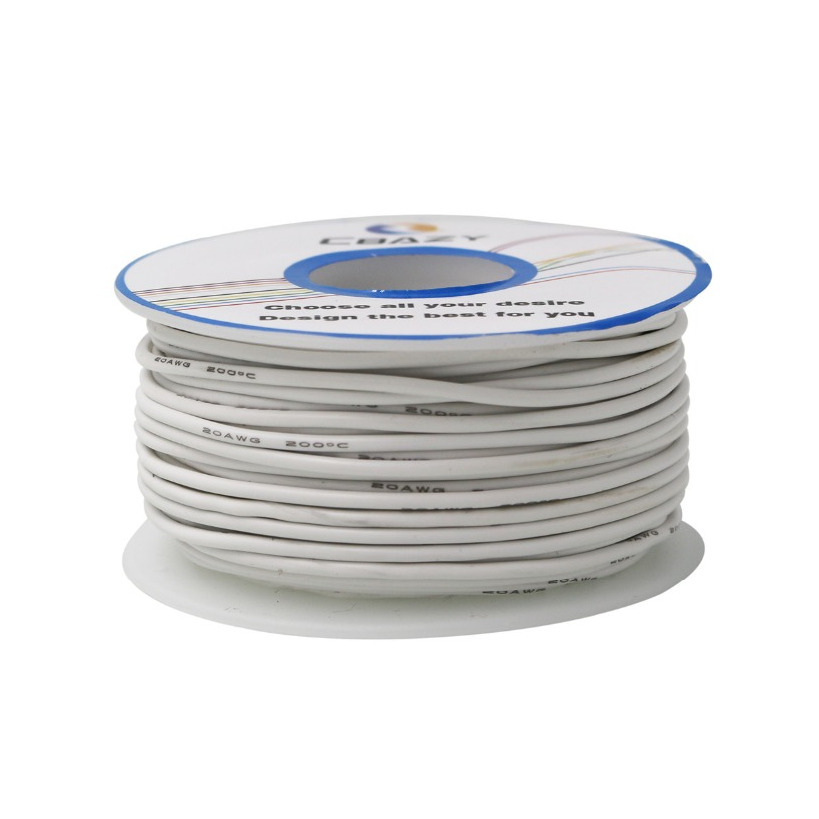
\includegraphics[width=5cm]{whitewire.jpg} }
& \begin{tabular}{l l}
\textbf{Manufacturer:} CBAZY & \textbf{Price per Inch:} \$0.02 \\
\textbf{Size:} 18AWG & \textbf{Cut Lengths:} 50.5"x2 \\
\textbf{Color:} White  & \textbf{Total Length:} 101" \\
\multicolumn{2}{p{8cm}}{\textbf{Description:} Stranded Hook-up Wire } \\
\end{tabular} \\

\parbox[c]{5cm}{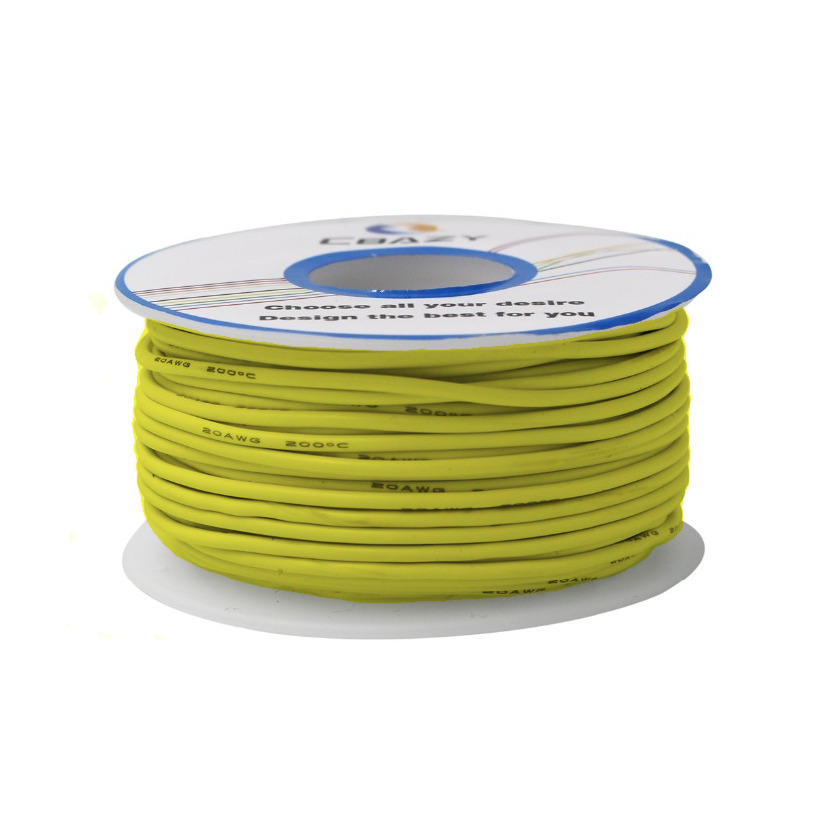
\includegraphics[width=5cm]{yellowire.jpg} }
& \begin{tabular}{l l}
\textbf{Manufacturer:} CBAZY & \textbf{Price per Inch:} \$0.02 \\
\textbf{Size:} 18AWG & \textbf{Cut Lengths:} 14"x2, 30.5x2" \\
\textbf{Color:} Yellow  & \textbf{Total Length:} 89" \\
\multicolumn{2}{p{8cm}}{\textbf{Description:} Stranded Hook-up Wire } \\
\end{tabular} \\

\parbox[c]{5cm}{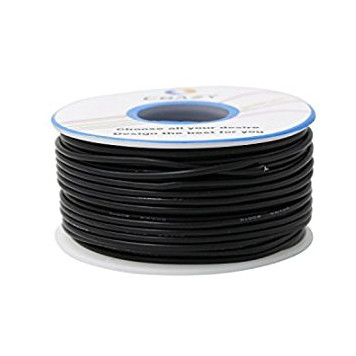
\includegraphics[width=5cm]{blackwire.jpg} }
& \begin{tabular}{l l}
\textbf{Manufacturer:} CBAZY & \textbf{Price per Inch:} \$0.02 \\
\textbf{Size:} 18AWG & \textbf{Cut Lengths:} 13"x2, 31.5x2" \\
\textbf{Color:} Black  & \textbf{Total Length:} 89" \\
\multicolumn{2}{p{8cm}}{\textbf{Description:} Stranded Hook-up Wire} \\
\end{tabular} \\

\parbox[c]{5cm}{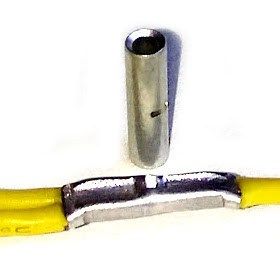
\includegraphics[width=5cm]{splice-terminal.jpg} }
& \begin{tabular}{l l}
\textbf{Manufacturer:} Ginsco & \textbf{Unit Price:} \$0.05 \\
\textbf{Size:} 14-16AWG & \textbf{Material:} Tinned Copper \\
\textbf{Description:} Splice terminal & \textbf{Quantity:} 2 \\
\end{tabular} \\

\parbox[c]{5cm}{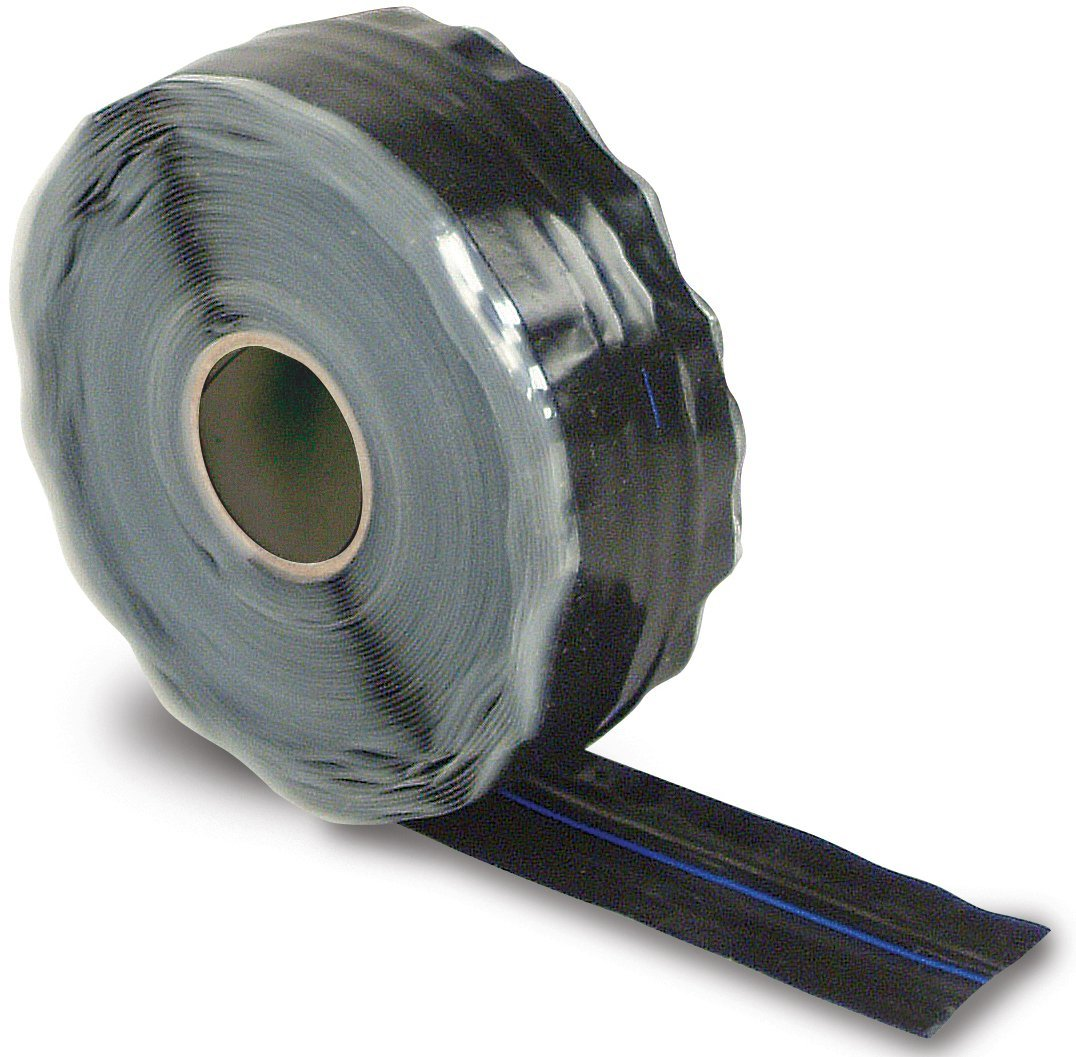
\includegraphics[width=5cm]{firetape.jpg} }
& \begin{tabular}{l l}
\textbf{Manufacturer:} DEI & \textbf{Unit Price:} \$30.63 \\
\textbf{Price Per Inch:} \$0.07 & \textbf{Total Length:} 20" \\
\textbf{Marketing Name:} Fire Tape & \textbf{Quantity:} 1 \\
\textbf{Width:} 1" & \textbf{Length:} 36' \\
\multicolumn{2}{p{10cm}}{\textbf{Description:} Self-Vulcanizing Silicone Rubber Tape} \\
\end{tabular} \\

\parbox[c]{5cm}{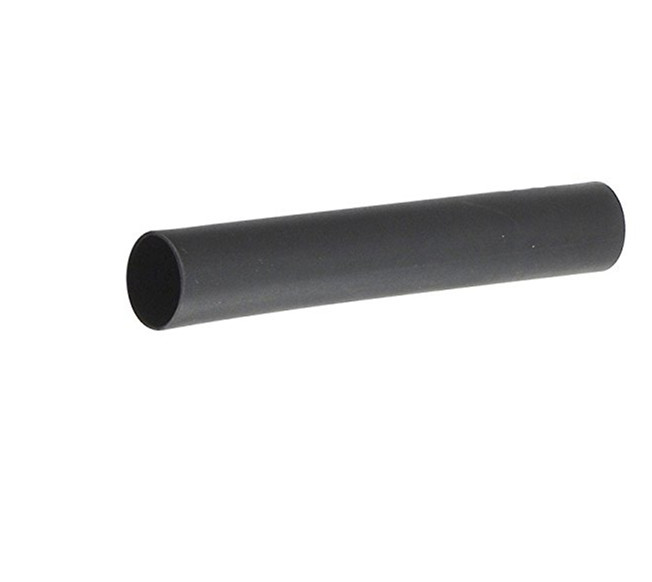
\includegraphics[width=5cm]{3by8shrinktube.jpg} }
& \begin{tabular}{l l}
\textbf{Manufacturer:} SES & \textbf{Price per Inch:} \$0.03 \\
\textbf{Diameter:} 3/8" & \textbf{Cut Lengths:} 1"x2 \\
\textbf{Color:} Black  & \textbf{Total Length:} 2" \\
\multicolumn{2}{p{10cm}}{\textbf{Description:} Dual-Wall Adhesive Heat Shrink Tube } \\
\end{tabular} \\

\parbox[c]{5cm}{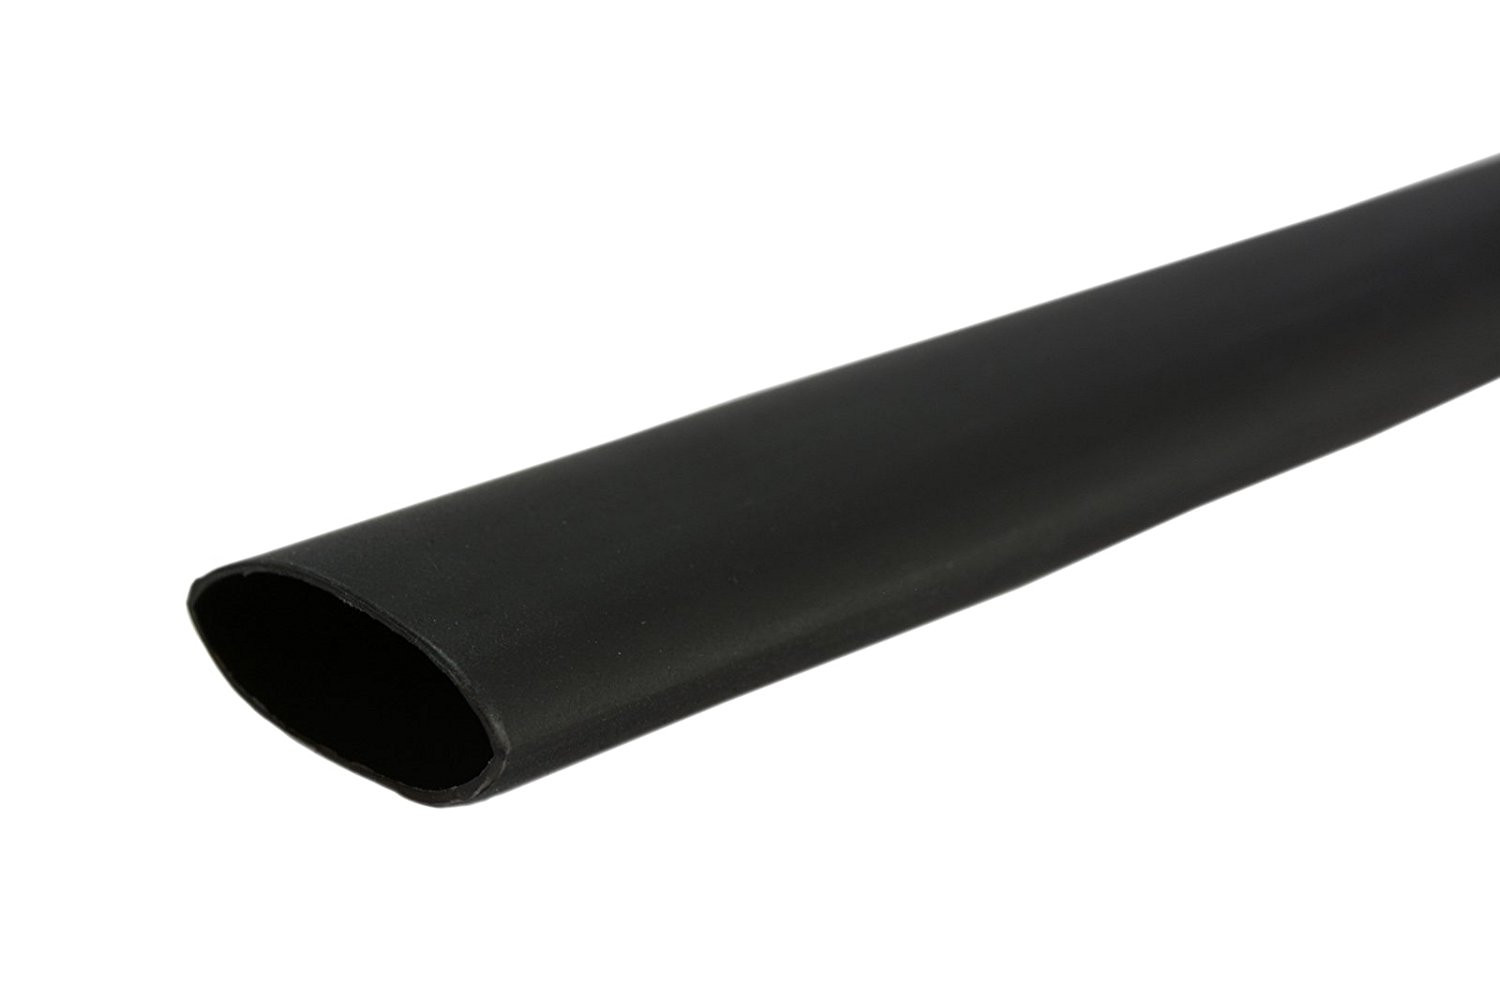
\includegraphics[width=5cm]{3by4shrinktube.jpg} }
& \begin{tabular}{l l}
\textbf{Manufacturer:} Temco & \textbf{Price per Inch:} \$0.13 \\
\textbf{Diameter:} 3/4" & \textbf{Cut Lengths:} 1.5"x4 \\
\textbf{Color:} Black  & \textbf{Total Length:} 6" \\
\multicolumn{2}{p{10cm}}{\textbf{Description:} Dual-Wall Adhesive Heat Shrink Tube } \\
\end{tabular} \\
% REDx2, GREENx2, BLUEx2 - 46"
% WHITEx2 - 51"
% Yellow 14"x2, 30.5
% Black 13", 31.5

& 
\begin{tabular}{l} 
\hline \\
\textbf{Total Cost Of Materials:} \$37.95 \\
\end{tabular} \\

\end{longtable}




% \begin{tabular}{c l l}
% \multirow{6}{*}{ \parbox[c]{4cm}{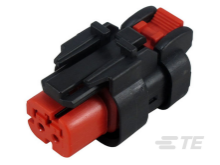
\includegraphics[width=4cm]{776427-1.png} } }
% & \multicolumn{1}{p{6cm}}{ 
% \textbf{Part Number: 776427-1} \newline
% \textbf{Manufacturer: TE Connectivity} \newline 
% \textbf{Number of Positions: } \newline 
% }
% & \multicolumn{1}{p{6cm}}{ 
% \textbf{Connector Style:} \newline 
% \textbf{Unit Price:} \newline 
% \textbf{Quantity:} \newline 
% \hline
% } \\
% \multirow{6}{*}{ \parbox[c]{4cm}{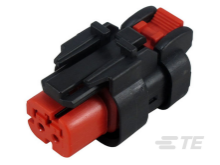
\includegraphics[width=4cm]{776427-1.png} } }
% & \multicolumn{1}{p{6cm}}{ 
% \textbf{Part Number: 776427-1} \newline
% \textbf{Manufacturer: TE Connectivity} \newline 
% \textbf{Number of Positions: } \newline 
% \textbf{Connector Style:} \newline 
% \textbf{Unit Price:} \newline 
% \textbf{Quantity:} \newline 
% } \\ 

% \end{tabular}

\section{Wiring Diagram}
The wiring diagram in Figure 3 on the next page specifies the exact connections that need to exist between different connector housings for the wiring harness to function.

\nopagebreak 
\begin{figure}[h]\label{fig:wiring}
\centering
\def\svgwidth{\columnwidth}
\input{wiringdiagram.pdf_tex}
\caption{Wiring diagram}
\end{figure}
\clearpage

\end{document}
